\section{Representation Generation Approach --- \ourSol}\label{sec:solution}
%In literature, there are three main approaches for solving multi-objective optimization problems: exact methods, meta-heuristic methods \cite{deb2001} and approximation methods \cite{ruzika2005approximation}. Exact methods aim to generate the entire Pareto front. {\color{red} i suggest to remove this paragraph, it seems to be not quite relevant here}
\vspace{-1mm}
The optimal feature selection problem is essentially a combinatorial problem. %Due to the non-convex nature of such problems, it is typically infeasible to obtain a closed-form representation of the Pareto front via CWMOIP \rev{[??]}. Further,
The number of non-dominant solutions grows exponentially along the number of features and objectives. Given its NP-hardness, it is neither practical nor necessary to find the entire true Pareto front \cite{koksalan2009multiobjective}. %as $\epsilon$-constraint approach and CWMOIP do.
Instead, obtaining a set of solutions that evenly distributed over the true Pareto front is representative, pragmatic and computationally referrable.

%\subsection{\ourSol~Method}\label{sec:solution:nc}
The normal constraint (NC) method \cite{normalCons} is an effective method in the literature that guarantees generating evenly distributed solutions over the entire Pareto front. The main idea of NC method is to use the \emph{utopia plane} to approximate the true Pareto front such that a set of evenly distributed reference points on \emph{utopia plane} would result to a set of evenly distributed solutions on Pareto front, after the projection along the normal vector of \emph{utopia plane}. Here, \emph{utopia plane} refers to the hyper plane determined by all the anchor points, each of which individually optimizes a single objective (e.g. $y_{1}^*$ for $y_1$-axis and $y_{2}^*$ for $y_2$-axis in Fig~\ref{fig:uhre}.a). However, the original NC method was developed on continuous solution space. In the case of IP, it can generate dominated solutions (see Fig~\ref{fig:uhre}.a) where point A is the solution generated using NC, but there exists a point B outside the shaded feasible region, dominating A. Therefore, we propose to combine the idea of \emph{utopia plane} and the $\epsilon$-constraint method such that all solutions are guaranteed to be non-dominant ones (see Fig~\ref{fig:uhre}.c).

\begin{figure}[t]
\vspace{-1mm}
\centering
%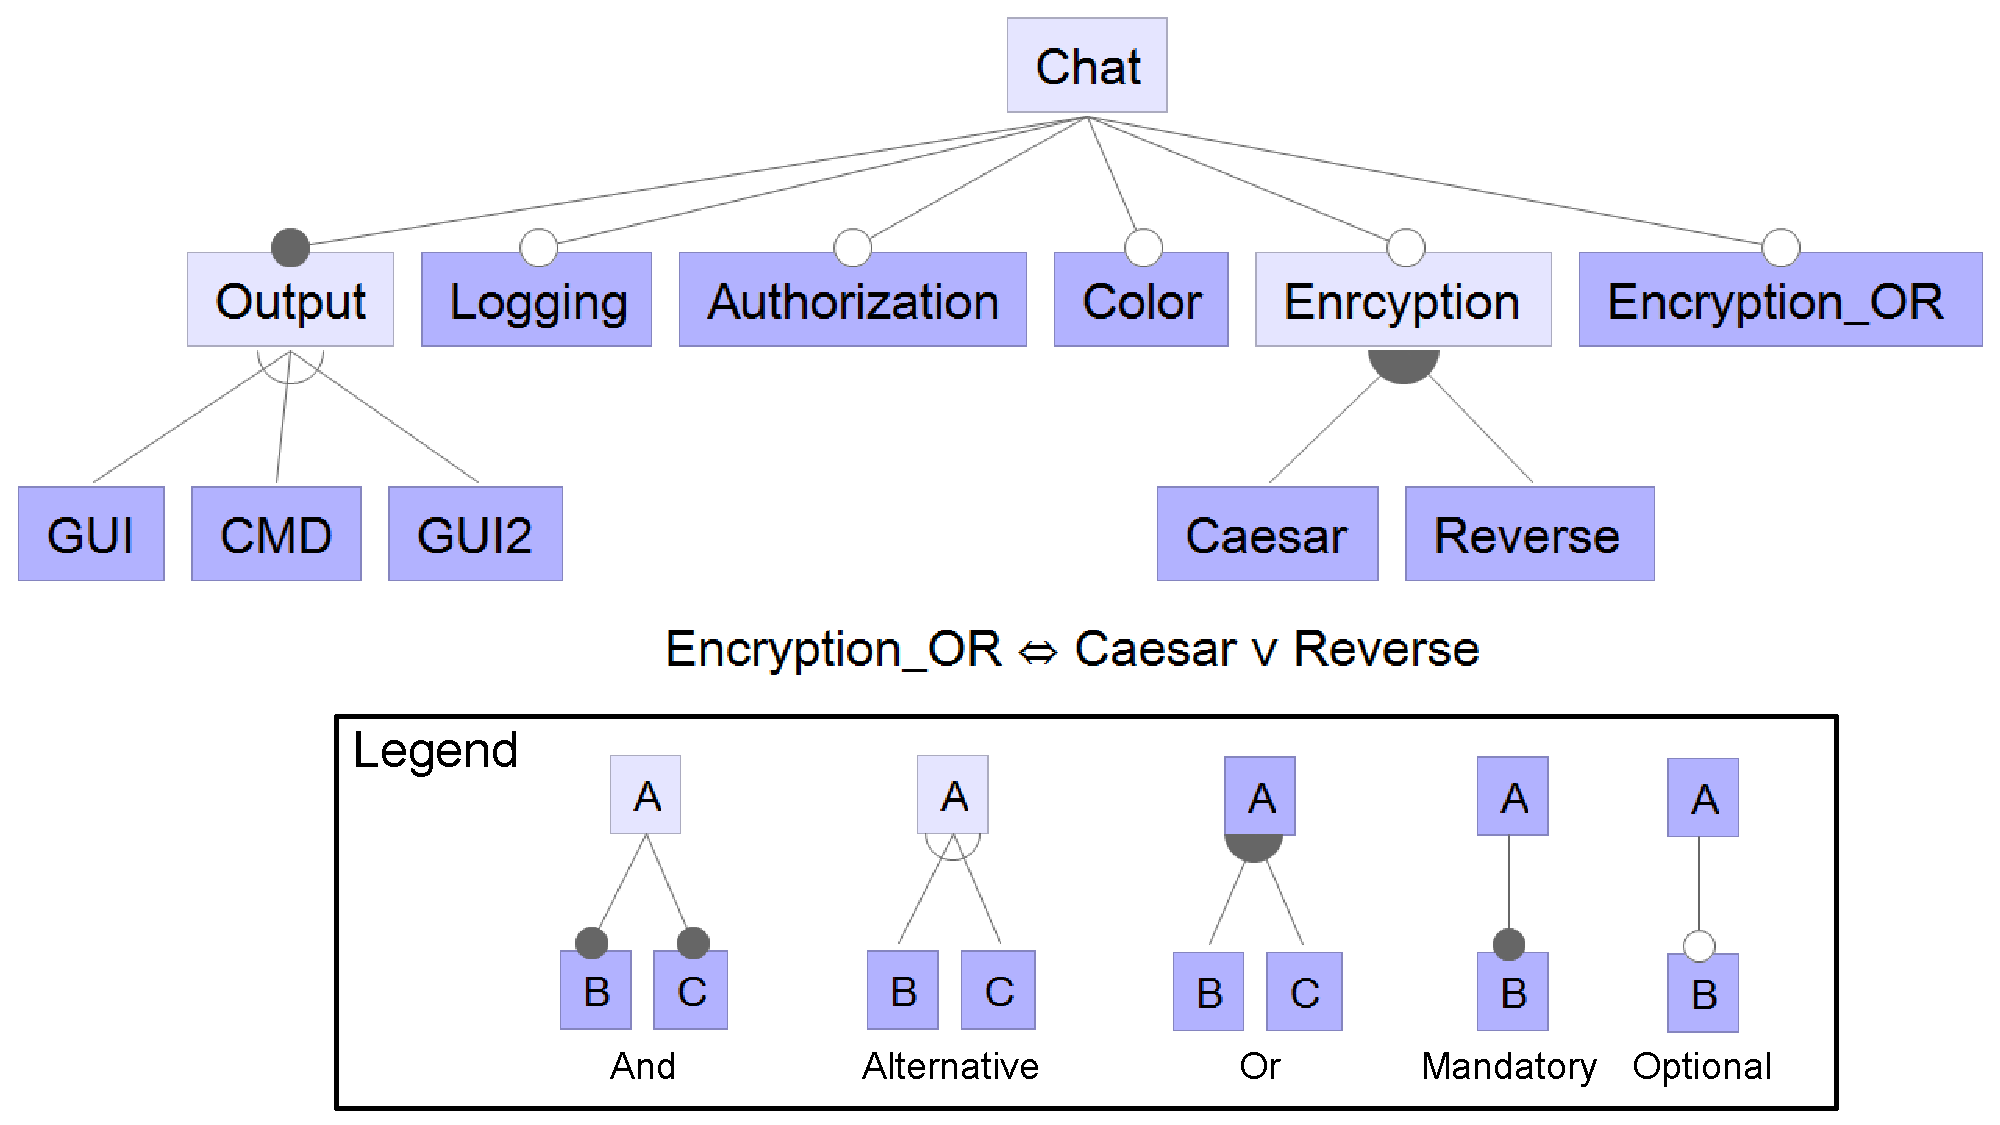
\epsfig{file=image/fm.bmp, width=8.5cm}
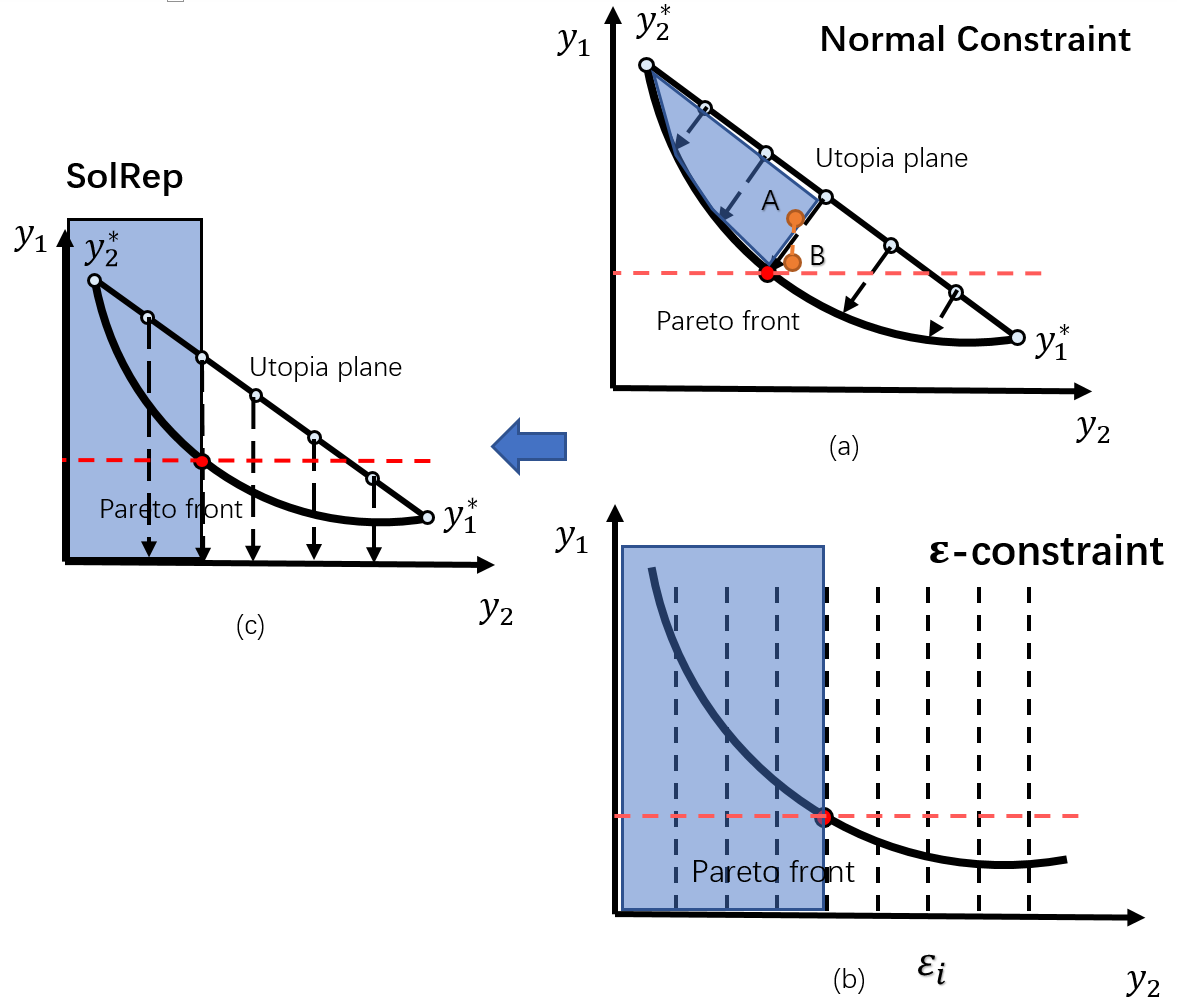
\includegraphics[width=8cm]{image/uhre.png}
\vspace{-3mm}
\caption{Two dimensional illustration of the proposed \ourSol~method}
\label{fig:uhre}
\end{figure}

Our proposed method consists of four main steps: 1) determine the utopia plane; 2) generate uniformly distributed reference points on the utopia plane; 3) for each reference point, use its $(k-1)$ coordinates to constrain the $(k-1)$ objectives; 4) optimize the $k$-th objective within the reduced solution space. Repeat steps 2) to 4) to achieve the representative Pareto front. In step 2), we resort to the hit-and-run (H\&R) method \cite{DBLP:journals/ior/Smith84} to sample the reference points.
%\rev{please insert this paper to reference list: Smith R L. Efficient Monte Carlo Procedures for Generating Points Uniformly Distributed Over Bounded Regions[J]. Operations Research, 1984, 32(6):1296-1308.}
Its principle is straightforward: let $p_{t}$ denote the current point then $p_{t+1} = p_{t} + \lambda*d$ is the next point, where $d$ is a random direction vector and $\lambda$ is the random length of the jump. As a random-walk algorithm, H\&R is proven to generate uniformly distributed points inside any polyhedron after a sufficient number of runs \cite{DBLP:journals/ior/Smith84}.

Note that an obvious alternative is to equally divide the Pareto front along each objective direction and then traverse each grid. However, it might not evenly cut the Pareto front and the computational efforts grow exponentially along the number of objectives.

\begin{algorithm}[t]                  % enter the algorithm environment
\caption{Function \small{\emph{SolRep()}} for $k$-objective IP}\label{alg:nchr}
\small
    %\KwIn{$M$: the feature model of the given system} %$maxIter$: the maximum number of iterations of the generation process
    \KwIn{$k$: the number of objectives, $N$: number of reference points, $X$: the set of linear constraints, $f_{i}$ coefficient vector of the $i$-th objective function}
    %\KwIn{$userInfor$: the contextual information of user device} %$maxIter$: the maximum number of iterations of the generation process
    \KwOut{$E$: the set of representative non-dominant solutions}
    %\KwOut{$returnedSol$: a solution returned to guide malware generation }
    \For{$ i = 1; i < k; i=i+1 $}{ \label{algo:nchr:i1}
    $y_{anch,i}= bintprog(X,f_{i})$\; \label{algo:nchr:i2}
    }
    $ ...$//determine the vertexes of utopia plane\; \label{algo:nchr:i3}
    $p_{0} = randPoint(y_{anch})$\; \label{algo:nchr:i4}
    $ ...$//generate a initial reference point $p_0$ on utopia plane\; \label{algo:nchr:i5}
    $P~\leftarrow~\emptyset, P = P \cup \{p_{0}\}$\; \label{algo:nchr:i6}
    \For{$ i = 1; i < N; i=i+1 $}{ \label{algo:nchr:i7}
    $d = randDirect(y_{anch})$\; \label{algo:nchr:i8}
    $\lambda_{range} = linprog(X,d,p_{0})$\; \label{algo:nchr:i9}
    $\lambda = unifrnd(\lambda_{range})$\; \label{algo:nchr:i10}
    $p_{0} = p_{0}+\lambda * d $\; \label{algo:nchr:i11}
    $P = P \cup \{p_{0}\}$\; \label{algo:nchr:i12}
    }
    $ ...$//find the other N-1 reference points\; \label{algo:nchr:i13}
    $E~\leftarrow~\emptyset$\; \label{algo:nchr:i14}
    \For{$ i = 1; i \le N; i=i+1 $}{ \label{algo:nchr:i15}
    $E = E \cup bintprog(X,f_{k},P_{i})$ \label{algo:nchr:i16}
    }
    \KwRet $E$;\label{algo:cwmoip:rt}
      %  $allMal\leftarrow allMal \cup newGeneration$\;\label{algo:cmb:23}

\end{algorithm}

The proposed \ourSol~method is presented in Algorithm \ref{alg:nchr}, which has the time complexity of $O(n)$ (consider $bintprog(X,f_{i})$ has $O(1)$, as a time limit is set for IP solving). The function $bintprog(X,f_{i})$ optimizes the $i$-th objective and returns one anchor point, $randPoint(y_{anch})$ generates a random initial reference point on utopia plane, $randDirect(y_{anch})$ returns a random direction vector, $linprog(X,d,p_{0})$ returns the upper and lower bounds of the jumping length $\lambda$, $unifrnd(\lambda_{range})$ returns one random length within the bounds, $bintprog(X,f_{k},P_{i})$ optimizes the $k$-th objective with the constraints incurred by the reference point $P_{i}$.
%As mentioned in Introduction Section, the drawbacks of meta-heuristic methods are: 1) non-guarantee of achieving the true Pareto optimal solutions; 2) the diversity of the obtained solutions over the entire solution space might not be guaranteed also.

%The normal boundary intersection (NBI) method \cite{das1998normal}. It generates non-Pareto and locally Pareto solutions \cite{messac2004normal}.
%The normal constraint (NC) method \cite{messac2004normal} guarantees the evenly distributed solutions over the entire Pareto front. In this method, the MOO problem is converted into one single objective optimization problem which is solved iteratively subject to a properly designed set of constraints. Different from the normal boundary intersection method, which requires the solutions being on the normal line.

%A comparative study by Messac et al. \cite{messac2003normalized} shows that NC performs favorably contrasting against NBI and physical programming. It is more computationally stable and is less likely trap to non-Pareto or locally Pareto solutions.

